\graphicspath{{Images/}}

\fontsize{9}{12}\selectfont{}
\singlespacing

\section{Appendix}
    \subsection{Glossary}
    \newglossaryentry{info_sci}{name=information science, description={- the study and practice of how to "collect, store, retrieve, and use information effectively"; explores the "social, ethical and cultural aspects of information"; combining "concepts and methods from various disciplines such as library science, computer science, linguistics, and psychology" \cite{bing_info_science}}}
    
    \newglossaryentry{info_rev}{name=information revolution, description={- "the radical changes wrought by computer technology on the storage of and access to information since the mid-1980s" \cite{info_rev}}}

    \newglossaryentry{moore}{name=Moore's law, description={- "the observation that the number of transistors in an integrated circuit... doubles about every two years" \cite{moore}}}
    
    \newacronym{nsa}{NSA}{- National Security Agency}
    
    \newacronym{nss}{NSS}{- National Security Systems; "systems that contain classified information or are otherwise critical to military or intelligence operations" \cite{nsm_10}}
    
    \newacronym{nist}{NIST}{- National Institute for Standards and Technology}
    
    \newacronym{dhs}{DHS}{- Department of Homeland Security}
    
    \newacronym{qc}{QC}{- quantum computer}
    
    \newacronym{pqc}{PQC}{- post-quantum cryptography}

    \newglossaryentry{moscas_theorem}{name=Mosca's theorem, description={- a theorem created by Michele Mosca that gives a "quantum threat timeline [to determine] whether a cyber-system is already at risk, well before the quantum threat has become concrete, because one has also to consider the needed migration time and the desired or required (e.g. by regulations) shelf-life time" \cite{quantum_threat_timeline}}}
    
    \newacronym{cisa}{CISA}{- Cybersecurity and Infrastructure Security Agency; an operational component of DHS}
    
    \newacronym{crqc}{CRQC}{- a cryptographically relevant quantum computer; a computer "capable of actually attacking real world cryptographic systems that would be infeasible to attack with a normal computer" \cite{nsa_pqc_faq}}
    
    \newacronym{ncf}{NCF}{- national critical functions; "functions of government and the private sector so vital to the United States that their disruption, corruption, or dysfunction would have a debilitating effect on security, national economic security, national public health or safety, or any combination thereof" \cite{ncfs}}
    
    \newacronym{fceb}{FCEB}{- Federal Civilian Executive Branch; often used to refer to ".gov" agencies}

    \newacronym{sltt}{SLTT}{- State/Local/Tribal/Territorial}

    \newacronym{ci}{CI}{- critical infrastructure}

    \newglossaryentry{entanglement}{name=entanglement, description={- the quantum state of each particle within a set cannot be described independently of the state of the other particles even when the particles are separated by a large distance; position, momentum, spin, and polarization may be all perfectly correlated \cite{entanglement}}}

    \newglossaryentry{qubit}{name=qubit, description={- a quantum bit}}

    \newglossaryentry{ket}{name=bra-ket notation, description={- sometimes referred to as Dirac notation, this is a special notation used in quantum mechanics to describe quantum states; its unique representation allows us to "compute probabilities, transition amplitudes, and other important quantities in quantum mechanics" \cite{dirac}}}

    \newglossaryentry{cia}{name=CIA triad, description={- the CIA triad defines the three key security objectives in cryptography; these are \gls{confidentiality}, gls{integrity}, and \gls{availability}; additional objectives of \gls{non-repudiation} and \gls{authenticity} are often considered sub-objective of integrity}}

    \newglossaryentry{confidentiality}{name=confidentiality, description={- information should not be divulged to unauthorized parties; only entities with express or explicit permission should be able to access information}}
    
    \newglossaryentry{integrity}{name=integrity, description={- information must not be modified or destroyed by outside parties or without authorization; sender and receivers of information should be able to trust the information sent or received has not and will not be tampered with or altered}}
    
    \newglossaryentry{non-repudiation}{name=non-repudiation, description={- actions should be uniquely traceable to the person or entity that did it}}
    
    \newglossaryentry{authenticity}{name=authenticity, description={- an entity is who they say they are; data has come from a trusted source}}
    
    \newglossaryentry{availability}{name=availability, description={- a system is available for use when needed and requested; can refer to timeliness and reliability}}

    \newglossaryentry{crypto}{name=cryptography, description={- the ability to send information between participants in a way that prevents others from reading it}}
    \newglossaryentry{q_crypto}{name=quantum cryptography, description={- cryptography that uses quantum mechanical phenomena to secure communication \cite{wiki_qcrypto}}}

    \newglossaryentry{attackvector}{name=attack vector, description={- "the method or combination of methods that cybercriminals use to breach or infiltrate a victim's network" \cite{attackvectors}}} 

    \newacronym{qkd}{QKD}{- quantum key distribution}

    \newglossaryentry{eavesdropping}{name=eavesdropping, description={- a passive attack where an adversary listens in on a information stream}}
    
    \newacronym{mitm}{MITM}{- a man-in-the-middle attack; an active attack where an adversary may "transmit their own messages, replay old messages, modify messages in transit, or delete or delay selected messages in transit" \cite{netsec}}

    \newacronym{otp}{OTP}{- one-time pad; a "single-use pre-shared key larger than or equal to size of the message being sent" that provides perfect secrecy, meaning it is technically impossible to crack \cite{wiki_otp}}

    \newglossaryentry{uncertainty}{name=Heisenberg uncertainty principle, description={- sometimes called the indeterminacy principles, it states "there is a limit to the precision with which certain pairs of physical properties, such as position and momentum, can be simultaneously known' \cite{uncertainty}}}

    \newacronym{dsa}{DSA}{- Digital Signature Algorithm}
    \newacronym{ecdsa}{ECDSA}{- Elliptic Curve Digital Signature Algorithm}
    \newacronym{ecdh}{ECDH}{- Elliptic Curve Diffie-Hellman}
    \newacronym{ecc}{ECC}{- Elliptic Curve Cryptography}
    \newacronym{rsa}{RSA}{- Rivest-Shamir-Adleman; an asymmetric encryption algorithm}

    \newglossaryentry{bruteforceattack}{name=brute-force attack, description={- an attack where an adversary tries all possible inputs to try to break into a system; on average, they must try about fifty percent before (i.e. passwords) before succeeding}}

    \newglossaryentry{preimageattack}{name=pre-image attack, description={- an attack where an attack tries to find a message which hashes to a specific value}}

    \newacronym{nsm}{NSM}{- National Security Memorandum}
    
    \newacronym{ics}{ICS}{- industrial control systems}
    
    \newacronym{cots}{COTS}{- commercial-off-the-shelf}

    \newacronym{sbom}{SBOM}{- Software Bill of Materials; likened to a ingredients list on a food label or receipt from the grocery store, this is an itemized and nested list of items that make up a software component that could be maintained for a vendor or given to potential consulting and contracting customers when building products, tools, and systems}

    \newglossaryentry{schrodinger}{name=Schr"\{o\}dinger's cat, description={- a thought experiment developed by Edwin Schr"\{o\}dinger in 1935 to criticize the Copenhagen interpretation of quantum mechanics; used to describe the quantum property of superposition, this scenario describes "a cat, a flask of poison, and a radioactive source connected to a Geiger counter" are placed in a sealed box, and until the box is opened, the cat may be both alive and dead at the same time}}
    
    \newglossaryentry{shor}{name=Shor's algorithm, description={- an algorithm devised by Peter Shoe in 1994 that is able to break the discrete log problem as well as the prime factorization problem}}
    
    \newglossaryentry{grover}{name=Grover's algorithm, description={- an algorithm devised by Lov Grover in 1996 capable of finding a unique input that was given to black box function when given its unique output, searching unstructured datasets with a polynomial speedup}}

    \newacronym{nistir}{NISTIR}{- NIST Interagency Report}
    
    \newacronym{aes}{AES}{- Advanced Encryption Standard}
    
    \newacronym{sha3}{SHA-3}{- Secure Hash Algorithm 3; an improved and more secure version of the SHA protocol}
    
    \newacronym{fips}{FIPS}{- Federal Information Processing Standards}
    \newacronym{sp}{SP}{- Special Publication}
    \newacronym{kem}{KEM}{- key encapsulation method; a method used "to secure symmetric key material for transmission using asymmetric (public-key) algorithms" \cite{wiki_kem}}

    \newglossaryentry{forwardsecrecy}{name=forward secrecy, description={- "session keys will not be compromised even if long-term secrets used in the session key exchange are compromised" \cite{wiki_forward}}}
    
    \newglossaryentry{sidechannelattack}{name=side-channel attack, description={- "any attack based on extra information that can be gathered because of the fundamental way a computer protocol or algorithm is implemented, rather than flaws in the design of the protocol or algorithm itself (e.g. flaws found in a cryptanalysis of a cryptographic algorithm)" \cite{wiki_sidechannel}}}
    
    \newacronym{fpu}{FPU}{- floating point unit}

    \printglossaries

% -------------------------------------------------------------

    \subsection{A Timeline} \label{timeline}
    \begin{figure}[h!]
        \centering
        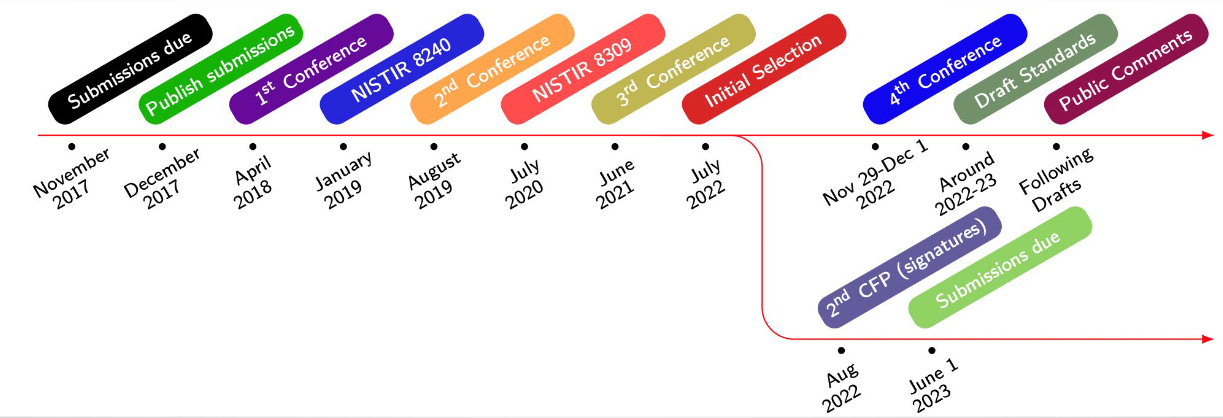
\includegraphics[width=1\linewidth]{Timeline.png}
        \caption{The latest timeline announced at the 4th PQC Standardization Workshop in 2023 \cite{moody_fourth}}
        \label{fig:timeline}
    \end{figure}

    \begin{table}[h!]
        \centering
        \begin{tabular}{cl}
             1801& Thomas Young's double-slit experiment kicks off field of quantum mechanics\\
     1935&Quantum entanglement discovered\\
     1935&Schr\"{o}dingers cat\\
     1955&Information science receives its name\\
     1965&Moore's law introduced\\
     1965&Stephen Weisner introduced conjugate coding\\
     1984&The BB84 protocol\\
     1994&Shor's algorithm\\
     1996&Grover's algorithm\\
     2015&NSA announcement\\
     2016&NIST announces PQC competition at PQCrypto\\
     2016&NIST releases NISTIR 8105, Report on PQC\\
     2016&NIST formal call for proposal\\
     2017&NIST deadline for submissions\\
     2017&IBM's 50-qubit quantum computer made\\
     2017&Round 1 algorithms announced\\
     2018&Intel's 49-qubit chip ``Tangle-Lake" made\\
     2018&Google's 72-qubit chip ``Bristlecone" made\\
     2018&NIST's first PQC standardization conference\\
     2019&Second round candidates announced\\
     2019&Deadline for updated packages for second round\\
     2019&Second PQC standardization conference\\
     2020&Third round candidates announced\\
     2020&Deadline for updated packages for third round\\
     2021&Third PQC standardization conference\\
     2022&Announcement of candidates to be standardized and fourth round candidates\\
     2022&Fourth PQC standardization conference\\
     2022&President of US releases NSM-8\\
     2023&Atom's 1180-qubit quantum computer made\\
     2023&President of US releases NSM-10\\
     2023&Three draft FIPS released for public comment\\
     2024&Fifth PQC standardization conference
        \end{tabular}
        \caption{A general timeline of quantum computing and NIST PQC standardization developments}
        \label{tab:qc_timeline}
    \end{table}
    
    \pagebreak
    
    \subsection{A Note on Polarizing Filters} \label{note:polarize}
    We have conceptualized qubits as photons with a spin in a particular direction or all possible directions in the case of superposition. If we were to compare a polarizing filter to a sieve, we might say that only photons with the same angle (or polarization) as the filter can get through the filter. But this is quantum physics, and in the case of qubits, it would be more accurate to say that if the polarization of the photon and filter match, all photons will get through; if they are opposite, none will get through; and if they are mismatch but not opposite (see Charles Bennett's definition of ``reliably distinguishable" in section \ref{superposition}), then a random number will get through the filter with the polarization possibly changed.

    \subsection{A Note on Symmetric Encryption}
    This paper has primarily focused on public key cryptography systems which are sometimes referred to as asymmetric key systems. An alternate type of encryption scheme is symmetric encryption. Research has indicated that these will be threatened by the development of a CRQC but not broken in the same way as public key systems, and as such, the increasing the length of keys for schemes such as AES and SHA-1/2/3 would be sufficient on the short term.